\chapter{Experiments and Results\label{ExperimentsResults}}

In this section, we introduce the test cases we intend to use. We go
through the details of our cosine and sum measure scoring schemes that
we will be using to test our systems ability to rank a correct disease
given a list of symptoms. This is followed by various test results
using different similarity measures and different matrix models. By
comparing the individual top scores of each measure on a given matrix,
stemmed or non-stemmed, we find the most efficient measure to score
data on our system. It should here be noted that each time we score a
given disease, we do it by taking the top 3000\footnote{A number
  chosen at random in between our total number of different diseases}
of the documents returned by the similarity measure and the Search
module. \\

We then look at ... Note: cluster and semantic section are still to
written. \\

Finally, we take discuss the potential noise of overview
articles\footnote{Articles found in / refering to many different
  diseases} and test the potential of concensus normalization.

\section{Test cases}

\textbf{BMJ} \\
In order to test our system we need to find some suitable test
cases that are not biased towards our own system. We have chosen to
first of all test our system against a subset of the disease cases in
\cite{HangwiTang11102006}, i.e. disease cases which can be found in
our system\footnote{As mentioned earlier in \ref{Database} our system
  can only help diagnose the diseases contained in the
  system}. However, there is one major difference between the tests
conducted by the people behind \cite{HangwiTang11102006} - they have a
medical background (a respiratory and sleep physician and a
rheumatologists) contrary to our computer science background. This
means that we have no bias or knowledge about selecting symptoms and,
as they explain, given some of the symptoms the correct diagnosis were
evident to them \cite{HangwiTang11102006}. Note that we will, in the
following sections, be reffering to the subset of the test cases in
\cite{HangwiTang11102006} as BMJ since this is were it was found. \\

The subset of the \cite{HangwiTang11102006} test cases include the
following 13 diseases:

\begin{table}[!h]
\caption{Disease / Symptoms list}
\begin{tabular}{|l|p{7cm}|}
\hline
Disease & Symptoms \\
\hline
Infective endocarditis & Acute, aortic,  regurgitation, depression,  abscess " \\
\hline
Cushing's syndrome & hypertension, adrenal, mass \\
\hline
Eosinophilic granuloma & Hip, lesion, older, child \\
\hline
Ehrlichiosis & fever, bilateral, thigh, pain, weakness \\
\hline
Neurofibromatosis type 1 & multiple, spinal, tumours, skin, tumours \\
\hline
Pheochromocytoma & hypertension, papilledema, headache, renal, mass, cafe, au, lait \\
\hline
Creutzfeldt-Jakob disease & ataxia, confusion, insomnia, death \\
\hline
Churg-Strauss syndrome & Wheeze, weight, loss, ANCA, haemoptysis, haematuria \\
\hline
Dermatomyositis & myopathy, neoplasia, dysphagia, rash, periorbital, swelling \\
\hline
Cat Scratch Disease & renal, transplant, fever, cat, lymphadenopathy \\
\hline
TEN & bullous, skin, conditions, respiratory, failure, carbamazepine \\
\hline
MELAS & seizure, confusion, dysphasia, T2, lesions \\
\hline
Brugada syndrome & cardiac arrest sleep \\
\hline
\end{tabular}
\end{table}

\textbf{Orphanet}
To examine significance of the test result, we have additionally selected some diseases at 'random' from Orpha.net. We require that the disease has a description on Orpha.net containing a sentence with 'characterized by'. Occationally we have meant that the 'characterized by' contained too many specific symptoms (e.g. derivatives of the name of the disease or a several sentences long list of symptoms) and have removed certain symptoms from the list. Examples of reductions would be\footnote{Note that this is based solely on our own judgement as non-physicians.} \\

congenital anomalies (microcephaly, specific facial characteristics, broad thumbs and halluces and postnatal growth retardation), intellectual deficit and behavioural characteristics \\

reduced to \\

congenital anomalies, intellectual deficit, behavioural \\

and  \\

congenital malformations: hydrocephalus (due to Dandy-Walker anomaly), cleft palate, and severe joint contractures \\

reduced to \\

congenital malformations: hydrocephalus, cleft palate, severe joint contractures \\

The test cases fetched from Orpha.net include the following 30 different diseases: 

\begin{table}[h]
\caption{Disease / symptom list 2}
\begin{tabular}{| p{5.5cm} | p{5.5cm} |}
\hline
Disease name & Symptom list \\
\hline
Apparent mineralocorticoid excess & early-onset, severe hypertension, associated, low renin levels, hypoaldosteronism \\
\hline
Rubinstein-Taybi syndrome & congenital anomalies, intellectual deficit, behavioural characteristics \\
\hline
Aagenaes syndrome & chronic severe lymphoedema, severe neonatal cholestasis, lessens during early childhood and becomes episodic \\
\hline
Aase Smith syndrome & congenital malformations: hydrocephalus, cleft palate, severe joint contractures \\
\hline
Achondroplasia & short limbs, hyperlordosis, short hands, macrocephaly, high forehead and saddle nose \\
\hline
Acalvaria & missing scalp and flat bones over an area of the cranial vault \\
\hline
Acrodysostosis & abnormally short and malformed bones of the hands and feet (peripheral dysostosis), nasal hypoplasia and mental retardation \\
\hline
Acromegaly & progressive somatic disfigurement (face and extremities) and systemic manifestations \\
\hline
Biliary atresia & biliary obstruction of unknown origin, neonatal period \\
\hline
Bronchiolitis obliterans with obstructive pulmonary disease & inflammatory and fibrosing thickening of bronchiolar walls, airflow obstruction \\
\hline
Cholera & severe diarrhea and vomiting \\
\hline
Choroideremia & progressive degeneration of the choroid, retinal pigment epithelium (RPE), and neural retina \\
\hline
Coats disease & abnormal development of retinal vessels (telangiectasia) with a progressive deposition of intraretinal or subretinal exudates \\
\hline
Omphalocele cleft palate syndrome lethal & omphalocele and cleft palate \\
\hline
Darier disease & keratotic papules in seborrheic areas and specific nail anomalies \\
\hline
Ichthyosis hepatosplenomegaly cerebellar degeneration & ichthyosis, hepatosplenomegaly and late-onset cerebellar ataxia \\
\hline
Emery-Dreifuss muscular dystrophy & muscular weakness and atrophy, with early contractures of the tendons and cardiomyopathy \\
\hline
\end{tabular}
\end{table}

\begin{table}[h]
\caption{Disease / symptom list 2, continuet}
\begin{tabular}{| p{5.5cm} | p{5.5cm}|}
\hline
Costello syndrome & postnatal growth retardation, coarse facies, intellectual deficit, skin anomalies and cardiac abnormalities \\
\hline
Fibrodysplasia ossificans progressiva & congenital malformation of great toes, progressive, disabling heterotopic osteogenesis in predictable anatomical patterns \\
\hline
Acropectorovertebral dysplasia & fusion of the carpal and tarsal bones, with complex anomalies of the fingers and toes \\
\hline
Osteogenesis imperfecta & increased bone fragility and low bone mass \\
\hline
Primary biliary cirrhosis & injury of the intrahepatic bile ducts \\
\hline
Hennekam syndrome & lymphoedema, intestinal lymphangiectasia, intellectual deficit and facial dysmorphism \\
\hline
Hyperlysinemia & elevated levels of lysine in the cerebrospinal fluid and blood \\
\hline
Jackson-Weiss syndrome & tarsal and/or metatarsal coalitions and variable craniosynostosis, accompanied by facial anomalies, broad halluces and normal hands \\
\hline
Jalili syndrome & amelogenesis imperfecta and cone-rod retinal dystrophy \\
\hline
Jeune syndrome & narrow thorax and short limbs \\
\hline
Multiple myeloma & overproduction of abnormal plasma cells in the bone marrow and manifested by skeletal destruction, bone pain, and presence of abnormous immunoglobulins \\
\hline
Trichodental syndrome & fine, dry and short hair with dental anomalies \\
\hline
\end{tabular}
\end{table}

\textbf{Blind tests}
In addition to the BMJ and Oprhanet test cases, we have performed a blind test on disease cases given by physician \cite{TheDude}.
>>Finish this section when ordentlig-syg results arrive!<<

\subsection{4.2 Scoring schemes}

As mentioned in the previous chapters, we will employ two different kinds of scoring measures - the cosine and sum measure. The original idea, behind using a sum measure, was to test how much the cosine measure would outperform this simpler measure but as we shall see in \ref{TestingCosineSimilarity} and \ref{TestingSumSimilarity}, the cosine measure is actually outperformed itself by the sum measure. We will try to explain this 'oddity' in the given section and for now focus the way we use the two different kinds of measure. The following cosine and sum score measures are described in accordance to how they function on the term document matrix. The exception of the disease matrix is described at the end of this section.

\subsubsection{4.2.1 The cosine score\label{CosineScore}}

We will be testing the following three different approaches to using
the cosine similarity measure: cosine mean, cosine median and cosine
max.\\

\textbf{Cosine mean}  \\
Every disease has one or more documents attached to it (as
described in \ref{Database}). This means that the same disease might
be returned many times when looking at a top score of document
similarity measures produced by e.g. the cosine score. Therefore, to
give each disease a score, we use a form of concensus method where we
sum the scores of each document belonging to that disease. This
produces a mean score of each disease. \\

When the system (or more specifically the Search module) receives a
query, it ranks the query vector of terms against all document vectors
in which one or more of the terms has appeared. This results in a list
of scores $\mathbb{x} = \left\{x_1, x_2, \dots, x_n \right\}$. It then
runs through every scored document and adds the score to the disease
from which the document came (in accordance to the concensus method
just described). Since some documents appear in more than one disease
(\ref{Database}), several diseases might have the sum of a single
document added to its score $\mathbb{x}_{\textrm{disease}_{1}} =
\left\{x_{\textrm{sum for} x_2, x_7, x_i, \dots, x_j}\right\}$,
$\mathbb{x}_{\textrm{disease}_{2}} = \left\{x_{\textrm{sum for} x_1,
  x_2, x_9, \dots, x_47, x_n}\right\}$.  Lastly, we evaluate the total
ranking of each disease. We combine each $x_{\textrm{disease}_1}$,
$x_{\textrm{disease}_2}$ into a list of all the returned disease
$\mathbb{SL} = \left\{x_{\textrm{disease}_1},x_{\textrm{disease}_2},
\dots, x_{\textrm{disease}_n}\right\}$. These are then sorted and the
highest scoring is deemed the most likely to be the correct disease
given the query vector. \\

\textbf{Cosine median} \\
The median is calculated much like the mean, except for selecting the median of $\mathbb{x}_{\textrm{disease}_{1}} = \left\{x_2,x_7, x_i, \dots, x_j\right\}, \mathbb{x}_{\textrm{disease}_{2}} = \dots, \mathbb{x}_{\textrm{disease}_{n}}$, instead of summing the scores as we did above. \\

\textbf{Cosine max} \\
Does the same as above, just selects the maximum scoring in each disease lists and sort the resulting list and select the highest scoring as the most probable.

\subsubsection{4.2.2 The sum score}

The sum measure works exactly like the cosine mean measure, except for running on non-normalized vectors. See \ref{VectorSimilarity} and \ref{SimpleSum} for further reasoning.

\subsubsection{4.2.3 The disease matrix exception}

This is simply a short note on how we use the cosine and sum measures on the disease matrix. The disease matrix has no document vectors and is solely made up of summed disease vectors. This means that there is no point in using cosine mean, median or max, as there is no multiple label occurences to run a concensus method over. Here the score is simply the cosine or sum measure calculated for each of the diseases that contain the queried term(s). \\

\subsection{4.3 Testing the cosine similarity measure\label{TestingCosineSimilarity}}

The first test we run is on for the three different cosine scoring measures - mean, median and max. On the two barcharts below \ref{termDoc_bmj_hist_3000_ns_mea_med_max_nc} and \ref{termDoc_orphan_hist_3000_ns_mea_med_max_nc} are shown the query scores of the BMJ and the Orhpa.net test cases. These are run on the non-stemmed term document matrix. The scores a drawn on a logarithmic scale while the 'real' scores a shown below each chart. Note that the values are 0-indexed(!) and all tests are performed on TF-IDF preprocessed matrices. \\


\begin{figure}[h!]
        \begin{center}
          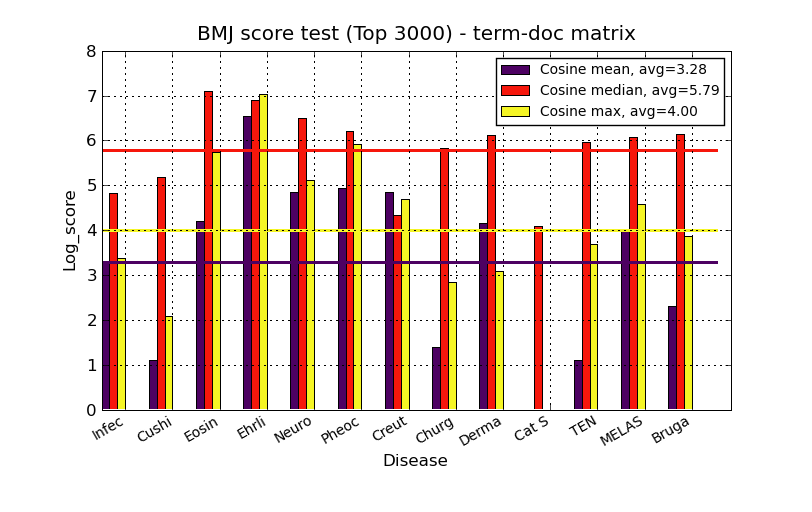
\includegraphics[width=0.9\textwidth]{termDoc_bmj_hist_3000_ns_mea_med_max_nc.png}
        \end{center}
        \caption{Test of non-stemmed mean, median and max using normalization and cosine}
        \label{termDoc_bmj_hist_3000_ns_mea_med_max_nc}
\end{figure}
 
Cosine: mean - Scores: [25, 2, 66, 692, 128, 139, 128, 3, 63, 0, 2, 52, 9] - In top 20: 5 \\
Cosine: median - Scores: [123, 179, 1210, 1004, 665, 502, 76, 343, 455, 59, 392, 430, 464] - In top 20: 0 \\
Cosine: max - Scores: [28, 7, 311, 1123, 166, 375, 109, 16, 21, 0, 39, 96, 47] - In top 20: 3

\begin{figure}[h!]
        \begin{center}
          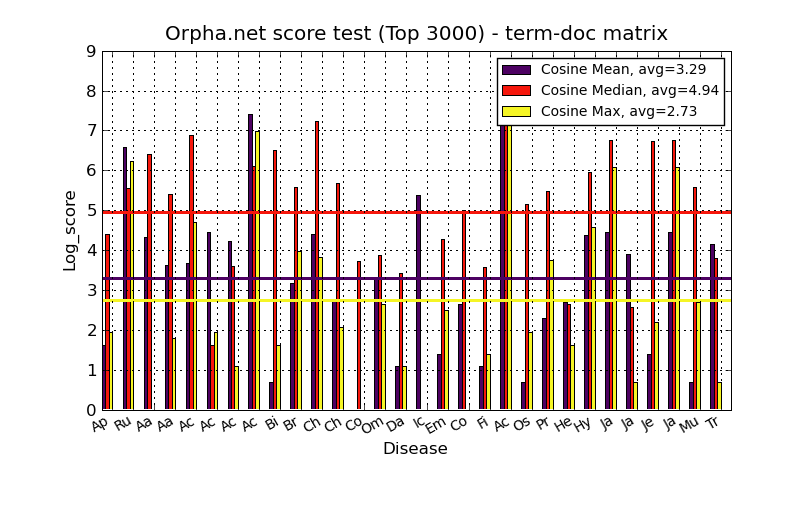
\includegraphics[width=0.9\textwidth]{barcharts/termDoc_orphan_hist_3000_ns_mea_med_max_nc.png}
        \end{center}
        \caption{Test of non-stemmed mean, median and max using normalization and cosine}
        \label{termDoc_orphan_hist_3000_ns_mea_med_max_nc}
\end{figure}
 
Cosine: mean - Scores: [4, 664, 30, 47, 38, 85, 62, 1371, 1, 32, 83, 15, 0, 26, 2, 81, 3, 16, 2, 3000, 4, 10, 13, 24, 66, 35, 3, 66, 4, 34] - In top 20: 13 \\
Cosine: median - Scores: [163, 357, 76, 240, 948, 4, 76, 141, 384, 314, 505, 211, 44, 181, 42, 773, 87, 169, 189, 3000, 179, 265, 21, 491, 692, 37, 435, 692, 358, 233] - In top 20: 1 \\
Cosine: max - Scores: [4, 858, 0, 10, 44, 15, 2, 541, 4, 116, 99, 18, 0, 6, 2, 0, 22, 0, 3, 3000, 9, 67, 5, 63, 201, 1, 8, 201, 9, 0] - In top 20: 19 \\

As we see here, the mean cosine measure performs best in the BMJ test set while the max cosine measure scores best in the Orpha.net test set. The median measure has an overall low score and running some quick tests on the different matrices, quickly reveals that median is not well suited as a measure to take into consideration. Therefore we will not be testing further on the cosine median score and continues with the two remaining scores from here on. Note that the AC score that has the worst performance in the Orpha.net test. It can and will happen that diseases are not found within the top 3000 documents that is returned. When this is the case, to avoid confusion in the bar charts and statistics, we simply set the score of any disease not found to a the high value of 3000, representing a bad performance. Note also that a missing bar, represents the top score 0. \\

We now continue testing the scoring measures, this time comparing the non-stemmed and stemmed term document matrices. The results are shown in the figures \ref{termDoc_bmj_hist_3000_ns_mea_s_mea_ns_max_s_max} and \ref{termDoc_orphan_hist_3000_ns_mea_s_mea_ns_max_s_max} below.

\begin{figure}[h!]
        \begin{center}
          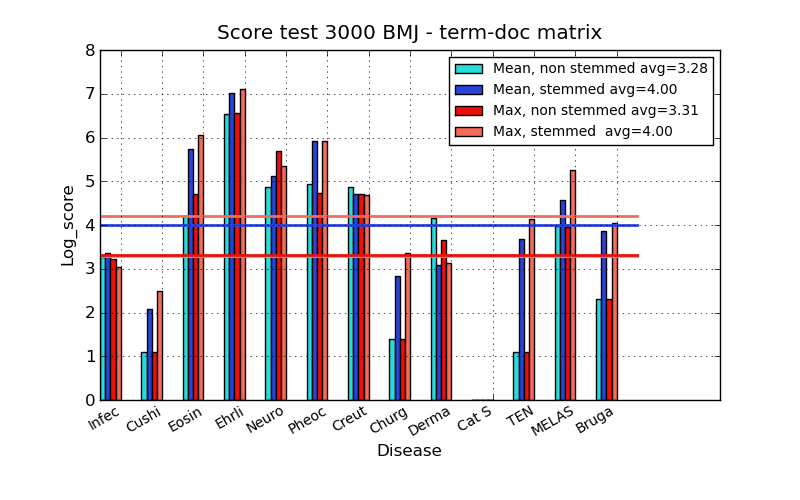
\includegraphics[width=0.9\textwidth]{barcharts/termDoc_bmj_hist_3000_ns_mea_s_mea_ns_max_s_max.png}
        \end{center}
        \caption{Test of non-stemmed mean, median and max using normalization and cosine}
        \label{termDoc_bmj_hist_3000_ns_mea_s_mea_ns_max_s_max}
\end{figure}

Cosine: mean non-stemmed - Scores: [25, 2, 66, 692, 128, 139, 128, 3, 63, 0, 2, 52, 9] - In top 20: 5 \\
Cosine: mean stemmed - Scores: [24, 2, 110, 710, 292, 113, 110, 3, 38, 0, 2, 51, 9] - In top 20: 5 \\
Cosine: max non-stemmed - Scores: [28, 7, 311, 1123, 166, 375, 109, 16, 21, 0, 39, 96, 47] - In top 20: 3 \\
Cosine: max stemmed - Scores [20, 11, 427, 1232, 210, 370, 108, 28, 22, 0, 62, 192, 56] - In top 20: 2

\begin{figure}[h!]
        \begin{center}
          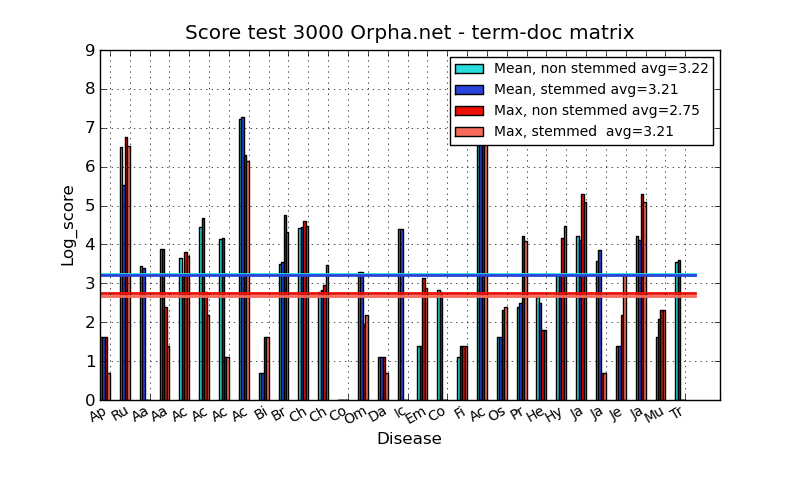
\includegraphics[width=0.9\textwidth]{barcharts/termDoc_orphan_hist_3000_ns_mea_s_mea_ns_max_s_max.png}
        \end{center}
        \caption{Test of non-stemmed mean, median and max using normalization and cosine}
        \label{termDoc_orphan_hist_3000_ns_mea_s_mea_ns_max_s_max}
\end{figure}
 
Cosine: mean non-stemmed - Scores: [4, 664, 30, 47, 38, 85, 62, 1371, 1, 32, 83, 15, 0, 26, 2, 81, 3, 16, 2, 3000, 4, 10, 13, 24, 66, 35, 3, 66, 4, 34] - In top 20: 13 \\
Cosine: mean stemmed - Scores: [4, 248, 29, 48, 23, 106, 64, 1436, 1, 34, 85, 16, 0, 26, 2, 81, 3, 15, 3, 3000, 4, 11, 11, 24, 60, 46, 3, 60, 7, 36] - In top 20: 13 \\
Cosine: max non-stemmed - Scores: [4, 858, 0, 10, 44, 15, 2, 541, 4, 116, 99, 18, 0, 6, 2, 0, 22, 0, 3, 3000, 9, 67, 5, 63, 201, 1, 8, 201, 9, 0] - In top 20: 19 \\
Cosine: max stemmed - Scores: [1, 677, 0, 3, 40, 8, 2, 462, 4, 75, 87, 31, 0, 8, 1, 0, 17, 0, 3, 3000, 10, 58, 5, 86, 162, 1, 24, 162, 9, 0] - In top 20: 18 \\

The two score tests just performed now presents us with a dilemma. In the BMJ test set the 'mean stemmed' and 'non-stemmed' scores performs best while in the Orpha.net test set, it is just the opposite. We have chosen to cope with this by taking out the top score measure for each of the test sets - 'mean non-stemmed' from BMJ and 'max stemmed' from the Orpha.net. \\

The next step is to analyse our data a bit by performing a square root transformation \ref{SquareRoot} of the TF-IDF preprocessed data above. Note that it is required that all values transformed are between 0 and 1, which in our case is secured by the fact that the matrices, we use for the cosine measure, are normalized. The reason for the square root analysis is that it allows us to see whether the data has been correctly weighted. The square root transformation raises small values by a greater degree than it does large values. This means that if our scores improve, the information containing terms in the term document matrix have not been given high enough values by the applied heuristics. \\

The tests are shown in the figures below, where we compare the best measures from above with their square root transformation.

\begin{figure}[h!]
        \begin{center}
          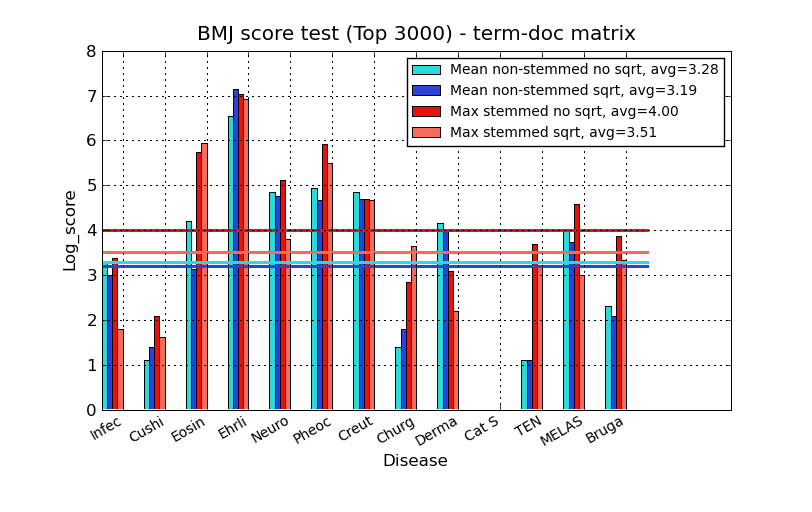
\includegraphics[width=0.9\textwidth]{barcharts/termDoc_bmj_hist_3000_ns_mea_ns_mea_sqr_s_max_s_max_sqr.png}
        \end{center}
        \caption{Test of non-stemmed mean, median and max using normalization and cosine}
        \label{termDoc_bmj_hist_3000_ns_mea_ns_mea_sqr_s_max_s_max_sqr}
\end{figure}

 
Cosine: mean non-stemmed - Scores: [25, 2, 66, 692, 128, 139, 128, 3, 63, 0, 2, 52, 9] - In top 20: 5 \\
Cosine: mean stemmed sqrt - Scores: [19,3,22,1268,115,105,108,5,54,0,2,41,7] - In top 20: 6 \\
Cosine: max non-stemmed - Scores: [20, 11, 427, 1232, 210, 370, 108, 28, 22, 0, 62, 192, 56] - In top 20: 2 \\
Cosine: max stemmed - Scores: [2, 10, 136, 1123, 68, 249, 130, 44, 8, 0, 47, 65, 25] - in top 20: 4

\begin{figure}[h!]
        \begin{center}
          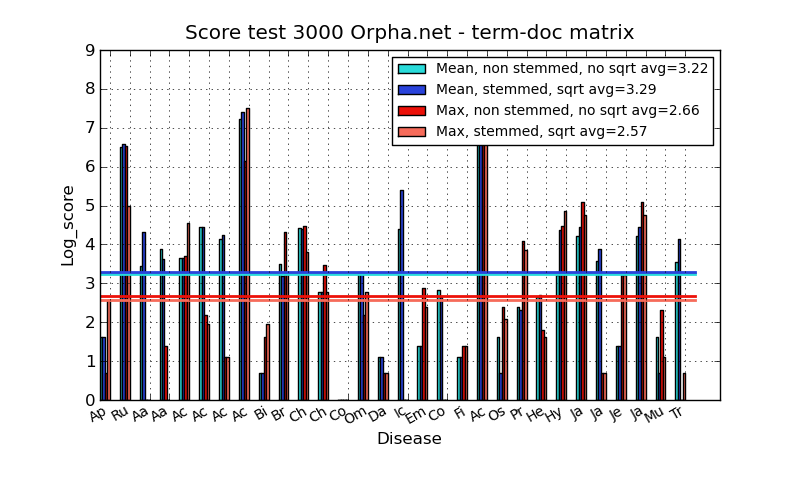
\includegraphics[width=0.9\textwidth]{barcharts/termDoc_orphan_hist_3000_ns_mea_ns_mea_sqr_s_max_s_max_sqr.png}
        \end{center}
        \caption{Test of non-stemmed mean, median and max using normalization and cosine}
        \label{termDoc_orphan_hist_3000_ns_mea_ns_mea_sqr_s_max_s_max_sqr}
\end{figure}

 
Cosine: mean non-stemmed - Scores: [4, 664, 30, 47, 38, 85, 62, 1371, 1, 32, 83, 15, 0, 26, 2, 81, 3, 16, 2, 3000, 4, 10, 13, 24, 66, 35, 3, 66, 4, 34] - In top 20: 13 \\
Cosine: mean stemmed sqrt - Scores: [4, 725, 75, 37, 38, 85, 68, 1651, 1, 23, 80, 15, 0, 26, 2, 218, 3, 13, 2, 3000, 1, 9, 14, 78, 84, 48, 3, 84, 1, 62] - In top 20: 13 \\
Cosine: max non-stemmed - Scores: [1, 677, 0, 3, 40, 8, 2, 462, 4, 75, 87, 31, 0, 8, 1, 0, 17, 0, 3, 3000, 10, 58, 5, 86, 162, 1, 24, 162, 9, 0] - In top 20: 18 \\
Cosine: max stemmed sqrt - Scores: [12, 145, 0, 0, 93, 6, 2, 1842, 6, 25, 44, 15, 0, 15, 1, 0, 10, 0, 3, 3000, 7, 46, 4, 128, 115, 1, 24, 115, 2, 1] - In top 20: 19 \\

These tests reveal some interesting results. Looking at the BMJ test set we see an overall improvement in the performance of the square root transformed measures. In Orpha.net test set there is an improvement in 'max stemmed' measure while a slight worsening of the 'mean non-stemmed' measure. However, there is no change in the number of top 20 results and the other measures shows a more significant improvement that the worsening of the last mentioned measure. Based on these results, we will not deny that the data in the TF-IDF matrices are not as optimized as could have been expected. But we can not say if these anomalies stem from the data or the calculations themselves. For now, we choose to view the square root transformation as a general improvement. \\

In section \ref{DiseaseMatrix}, we will be using the best measure of the cosine scoring tests executed above - the 'mean stemmed sqrt' and the 'max stemmed sqrt' cosine similarity measures.

\subsection{4.4 Testing the sum similarity measure\label{TestingSumSimilarity}}

In this section, we the same tests as described in the previous section, except for the square root transformation which makes no sense since we will be running on unnormalized data. Or in other word on values above and below 1 \ref{SquareRoot}. The first test is run for the mean, median and max sum measures on a TF-IDF non-normalized term document matrix. The results are shown on the figures \ref{termDoc_bmj_hist_3000_sum_mea_med_max} below. 

\begin{figure}[h!]
        \begin{center}
          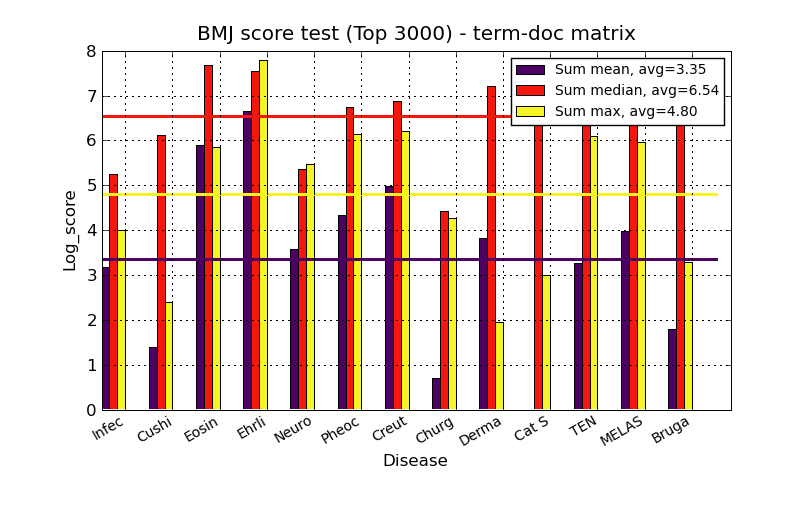
\includegraphics[width=0.9\textwidth]{barcharts/termDoc_bmj_hist_3000_sum_mea_med_max.png}
        \end{center}
        \caption{Test of non-stemmed mean, median and max using normalization and cosine}
        \label{termDoc_bmj_hist_3000_sum_mea_med_max}
\end{figure}

Sum: mean - Scores: [23, 3, 362, 772, 35, 76, 144, 1, 45, 0, 25, 53, 5] - In top 20: 4 \\
Sum: median - Scores: [188, 459, 2150, 1878, 213, 852, 974, 83, 1353, 670, 2193, 689, 1210] - In top 20: 0 \\
Sum: max - Scores: [54, 10, 344, 2401, 235, 469, 495, 70, 6, 19, 441, 391, 26] - In top 20: 3

\begin{figure}[h!]
        \begin{center}
          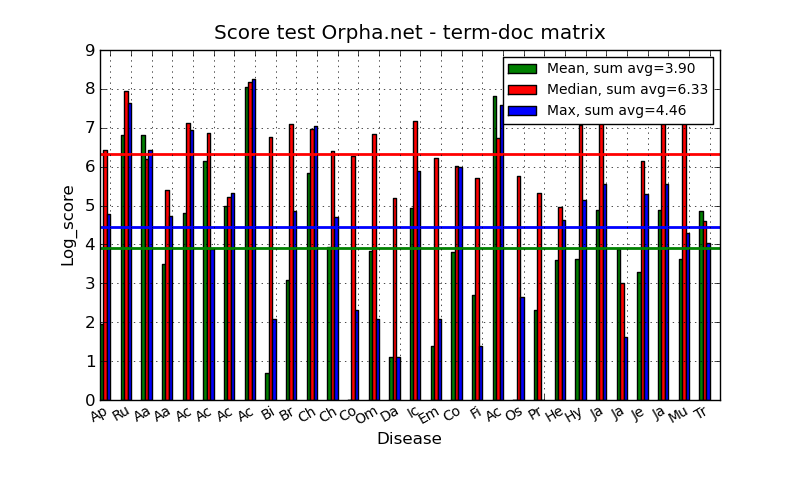
\includegraphics[width=0.9\textwidth]{barcharts/termDoc_orphan_hist_3000_ns_mea_med_max_sum.png}
        \end{center}
        \caption{Test of non-stemmed mean, median and max using normalization and cosine}
        \label{termDoc_orphan_hist_3000_ns_mea_med_max_sum}
\end{figure}
 
Sum: mean - Scores: [6, 910, 917, 32, 122, 460, 145, 3119, 1, 21, 342, 50, 0, 45, 2, 137, 3, 44, 14, 2458, 0, 9, 36, 37, 132, 47, 26, 132, 37, 127] - In top 20: 8 \\
Sum: median - Scores: [626, 2814, 495, 219, 1232, 963, 182, 3590, 872, 1207, 1056, 595, 526, 940, 179, 1292, 503, 408, 304, 845, 320, 204, 143, 1165, 1763, 19, 467, 1763, 1532, 100] - In top 20: 1 \\
Sum: max - Scores: [119, 2081, 611, 113, 1031, 48, 203, 3833, 7, 127, 1139, 109, 9, 7, 2, 357, 7, 401, 3, 1957, 13, 0, 102, 169, 260, 4, 198, 260, 72, 55] - In top 20: 9 \\

Like in the previous section, we again see the poor results given by the median measure and discards this for further testing. In the next test we compare the mean and sum measure in the stemmed and non-stemmed matrices. The tests are shown on the figures \ref{termDoc_bmj_hist_3000_ns_s_mea_max_sum} and \ref{termDoc_orphan_hist_3000_ns_s_mea_max_sum}.

\begin{figure}[h!]
        \begin{center}
          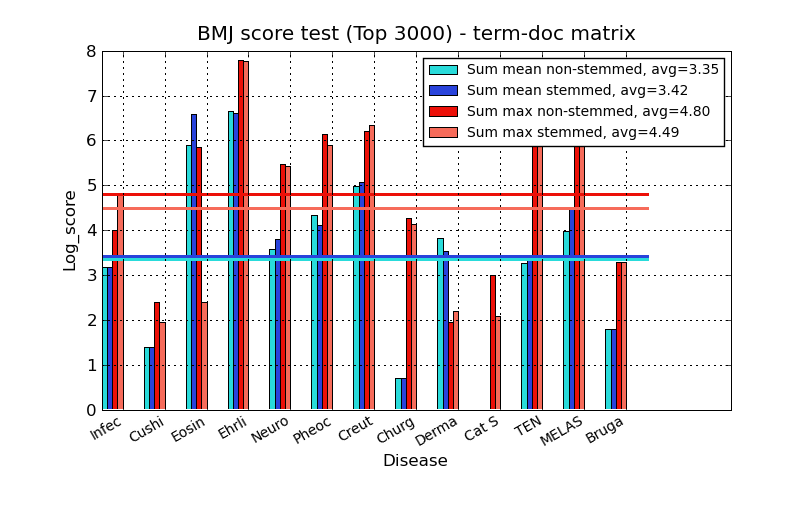
\includegraphics[width=0.9\textwidth]{barcharts/termDoc_bmj_hist_3000_ns_s_mea_max_sum.png}
        \end{center}
        \caption{Test of non-stemmed mean, median and max using normalization and cosine}
        \label{termDoc_bmj_hist_3000_ns_s_mea_max_sum}
\end{figure} 

Sum: mean non-stemmed - Scores: [23, 3, 362, 772, 35, 76, 144, 1, 45, 0, 25, 53, 5] - In top 20: 4 \\
Sum: mean stemmed - Scores: [23, 3, 720, 746, 44, 60, 158, 1, 33, 0, 27, 88, 5] - In top 20: 4 \\
Sum: max non-stemmed - Scores: [54, 10, 344, 2401, 235, 469, 495, 70, 6, 19, 441, 391, 26] - In top 20: 3 \\
Sum: max stemmed - Scores: [120, 6, 10, 2374, 228, 360, 566, 62, 8, 7, 394, 496, 26] - In top 20: 4

\begin{figure}[h!]
        \begin{center}
          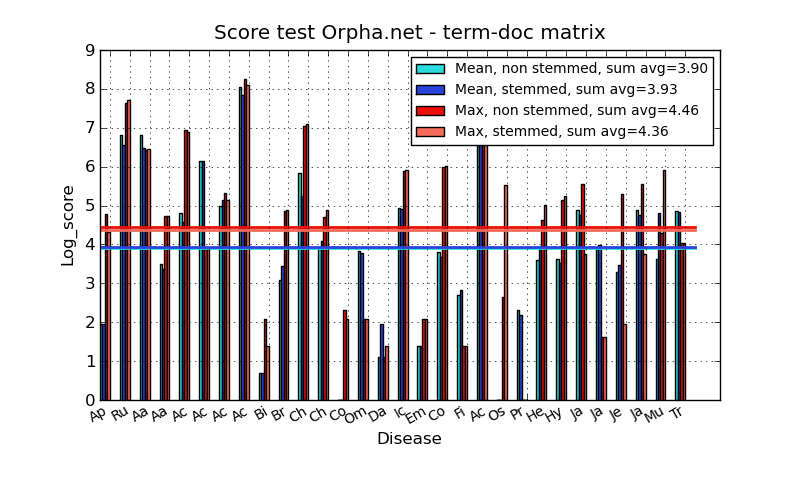
\includegraphics[width=0.9\textwidth]{barcharts/termDoc_orphan_hist_3000_ns_s_mea_max_sum.png}
        \end{center}
        \caption{Test of non-stemmed mean, median and max using normalization and cosine}
        \label{termDoc_orphan_hist_3000_ns_s_mea_max_sum}
\end{figure} 
 
Sum: mean non-stemmed - Scores: [6, 910, 917, 32, 122, 460, 145, 3119, 1, 21, 342, 50, 0, 45, 2, 137, 3, 44, 14, 2458, 0, 9, 36, 37, 132, 47, 26, 132, 37, 127] - In top 20: 8 \\
Sum: mean stemmed - Scores: [6, 708, 644, 28, 97, 460, 170, 2522, 1, 30, 190, 58, 0, 43, 6, 136, 3, 39, 16, 2636, 0, 8, 50, 33, 115, 53, 31, 115, 121, 124] - In top 20: 8 \\
Sum: max non-stemmed - Scores: [119, 2081, 611, 113, 1031, 48, 203, 3833, 7, 127, 1139, 109, 9, 7, 2, 357, 7, 401, 3, 1957, 13, 0, 102, 169, 260, 4, 198, 260, 72, 55] - In top 20: 9 \\
Sum: max stemmed - Scores: [75, 2228, 638, 113, 993, 48, 171, 3281, 3, 131, 1194, 131, 7, 7, 3, 365, 7, 414, 3, 2242, 253, 0, 150, 188, 42, 4, 6, 42, 372, 55] - In top 20: 9 \\

We see here that the 'mean sum' similarity measure clearly outperforms the 'max sum'. In section \ref{DiseaseMatrix}, we compare this measure with the best of the cosine measure on and the term document and disease matrices.

\subsection{4.5 The disease and term document matrix - cosine,  and sum and final result}

Now that we have found the results for the best measures to be used on the term document matrix, we focus our attention on the disease matrix. We will in the following be testing the sum and cosine measure on the disease matrix and, in the end of the section, compare these results to that of the term document. \\

In the first test, we look at the performance of the cosine (mean), cosine-sqrt and the sum measure on the BMJ and Orpha-net test sets. These test are performed on both the non-stemmed and stemmed. The results are shown on the figures \ref{diseaseMatrix_bmj_hist_norm_3000_ns_cos_sqrt_cos_sum_nn}, \ref{diseaseMatrix_orphan_hist_NOTnorm_3000_ns_cos_sqrt_cos_sum_nn}, \ref{diseaseMatrix_bmj_hist_norm_3000_s_cos_sqrt_cos_sum_nn} and \ref{diseaseMatrix_orphan_hist_NOTnorm_3000_s_cos_sqrt_cos_sum_nn} below: \\

Non-stemmed:

\begin{figure}[h!]
        \begin{center}
          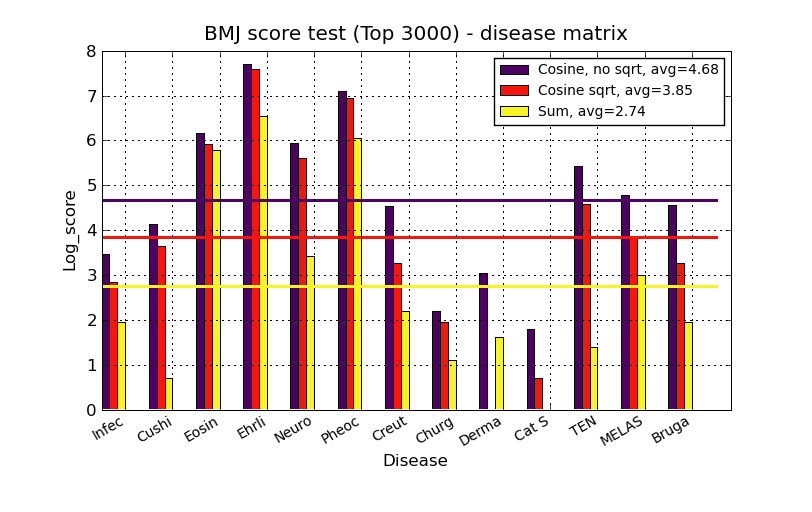
\includegraphics[width=0.9\textwidth]{barcharts/diseaseMatrix_bmj_hist_norm_3000_ns_cos_sqrt_cos_sum_nn.png}
        \end{center}
        \caption{Test of non-stemmed mean, median and max using normalization and cosine}
        \label{diseaseMatrix_bmj_hist_norm_3000_ns_cos_sqrt_cos_sum_nn}
\end{figure}
 
Cosine - Scores: [31,62,474,2220,377,1225,93,8,20,5,227,118,94] - In top 20: 2 \\
Cosine sqrt - Scores: [16,37,375,2001,270,1037,25,6, 0,1, 97, 45,25] - In top 20: 4 \\
Sum - Scores: [ 6,1,323, 691,30,427,8,2,4,0,3,19,6] - In top 20: 9 \\

\begin{figure}[h!]
        \begin{center}
          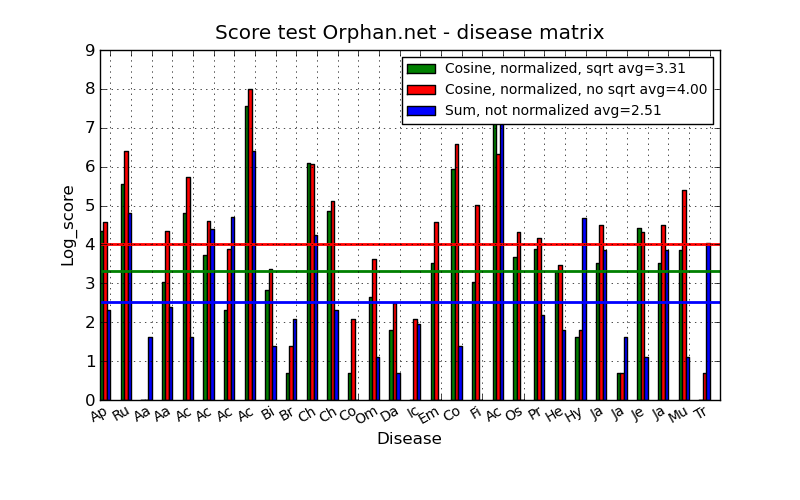
\includegraphics[width=0.9\textwidth]{barcharts/diseaseMatrix_orphan_hist_NOTnorm_3000_ns_cos_sqrt_cos_sum_nn.png}
        \end{center}
        \caption{Test of non-stemmed mean, median and max using normalization and cosine}
        \label{diseaseMatrix_orphan_hist_NOTnorm_3000_ns_cos_sqrt_cos_sum_nn}
\end{figure}
 
Cosine - Scores:[95,599,0,76,307,99,47,2989,28,3,430,165,7,37,11,7,97,717,150, 562,74,64,31,5,89,1,75,89,222,1] - In top 20: 8 \\
Cosine sqrt - Scores: [76,257,0,20,122,41, 9,1912,16,1,448,128,1,13, 5,0,33,380, 20,1687,39,47,26,4,33,1,83,33, 46,0] - In top 20: 11 \\
Sum - Scores: [9,123,4,10,4,81,109,601,3,7,68,9,0,2,1, 6,0,3,0,3000,0,8, 5,107,46,4,2,46,2,55] - In top 20: 20 \\

Stemmed:

\begin{figure}[h!]
        \begin{center}
          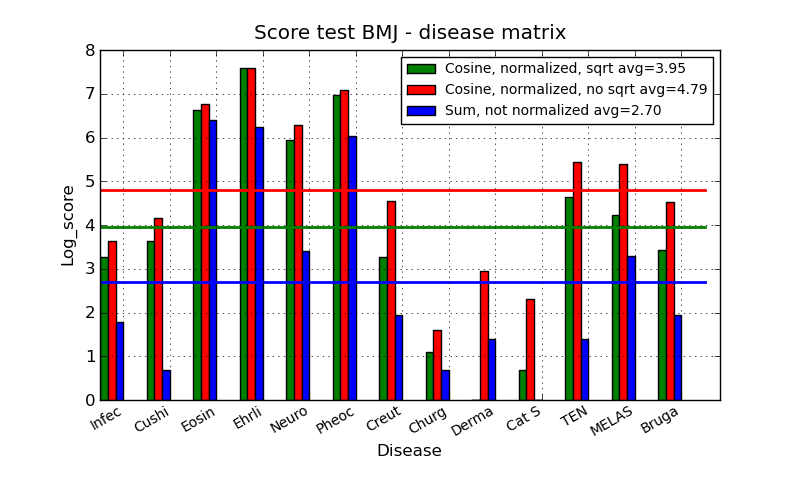
\includegraphics[width=0.9\textwidth]{barcharts/diseaseMatrix_bmj_hist_norm_3000_s_cos_sqrt_cos_sum_nn.png}
        \end{center}
        \caption{Test of non-stemmed mean, median and max using normalization and cosine}
        \label{diseaseMatrix_bmj_hist_norm_3000_s_cos_sqrt_cos_sum_nn}
\end{figure}

 
Cosine stemmed - Scores: [37,63,872,1963,533,1198,93,4,18,9,230,221,91] - In top 20: 3 \\
Cosine sqrt stemmed - Scores: [25,37,748,1970,384,1053,25,2, 0,1,102, 68,30] - In top 20: 3 \\
Sum stemmed - Scores: [5,1,597,511,29,413,6,1,3,0,3,26,6] - In top 20: 8

\begin{figure}[h!]
        \begin{center}
          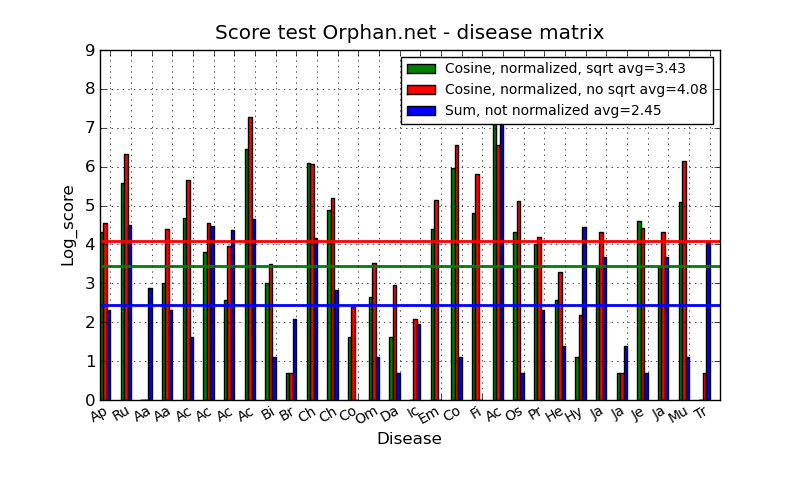
\includegraphics[width=0.9\textwidth]{barcharts/diseaseMatrix_orphan_hist_NOTnorm_3000_s_cos_sqrt_cos_sum_nn.png}
        \end{center}
        \caption{Test of non-stemmed mean, median and max using normalization and cosine}
        \label{diseaseMatrix_orphan_hist_NOTnorm_3000_s_cos_sqrt_cos_sum_nn}
\end{figure}

 
Cosine stemmed - Scores: [94,553,0,80,284,94,51,1454,32,1,433,181,10,33,18,7,169,710,334, 704,167,65,26,8,74,1,83,74,468,1] - In top 20: 8 \\
Cosine sqrt stemmed - Scores: [74,263,0,19,106,44,12, 635,19,1,446,133, 4,13, 4,0, 80,391,122,2137, 74,54,12,2,30,1,99,30,162,0] - In top 20: 13 \\
Sum stemmed - Scores: [9,90,17, 9,4,86,79,105,2,7,64,16,0,2,1, 6,0,2,0,3000,1,9,3, 84,39,3,1,39,2,59] - In top 20: 20 \\

When it comes to scoring diseases on in the disease matrix, the sum measure greatly outrival the cosine measure, with or without the square root transformation. If we look at the average values of the returned results, it seems that the stemmed version of the disease matrix is the best choice for optimized performance. \\

For the final test of measure and model, we compare the top results of the two matrices - term document and disease matrix. We will compare the different scores from the stemmed version of both matrix types since this seems to provide the overall best performance. In the figures \ref{termDoc_bmj_hist_3000_sum_dm_mea_cos_sqrt_td_max_cos_sqrt_td_mea_sum_td} and \ref{termDoc_orphan_hist_3000_sum_dm_mea_cos_sqrt_td_max_cos_sqrt_td_mea_sum_nn_td} below are bar chart of the best scores found for the prototype system:

\begin{figure}[h!]
        \begin{center}
          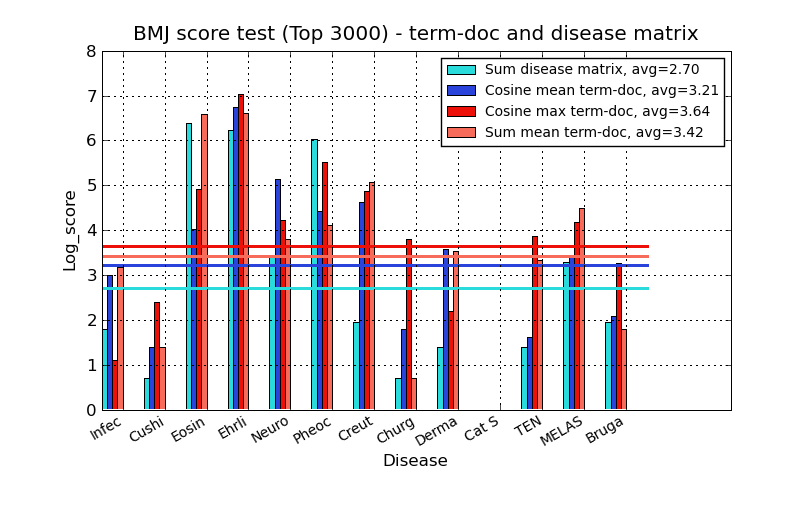
\includegraphics[width=0.9\textwidth]{barcharts/termDoc_bmj_hist_3000_sum_dm_mea_cos_sqrt_td_max_cos_sqrt_td_mea_sum_td.png}
        \end{center}
        \caption{Test of non-stemmed mean, median and max using normalization and cosine}
        \label{termDoc_bmj_hist_3000_sum_dm_mea_cos_sqrt_td_max_cos_sqrt_td_mea_sum_td}
\end{figure}
 
Sum: disease matrix - Scores: [ 6,1,323, 691,30,427,8,2,4,0,3,19,6] - In top 20: 9 \\
Cosine: mean stemmed sqrt - Scores: [19,3,22,1268,115,105,108,5,54,0,2,41,7] - In top 20: 6 \\
Cosine: max stemmed - Scores: [2, 10, 136, 1123, 68, 249, 130, 44, 8, 0, 47, 65, 25] - in top 20: 4 \\
Sum: term-doc mean - Scores: [23, 3, 720, 746, 44, 60, 158, 1, 33, 0, 27, 88, 5] - In top 20: 4

\begin{figure}[h!]
        \begin{center}
          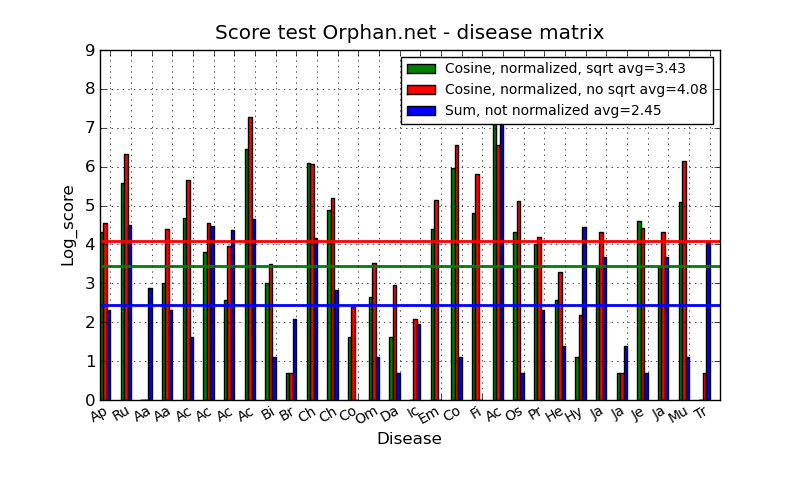
\includegraphics[width=0.9\textwidth]{barcharts/diseaseMatrix_orphan_hist_NOTnorm_3000_s_cos_sqrt_cos_sum_nn.png}
        \end{center}
        \caption{Test of non-stemmed mean, median and max using normalization and cosine}
        \label{termDoc_orphan_hist_3000_sum_dm_mea_cos_sqrt_td_max_cos_sqrt_td_mea_sum_nn_td}
\end{figure}

Sum: disease matrix - Scores: [9,90,17, 9,4,86,79,105,2,7,64,16,0,2,1, 6,0,2,0,3000,1,9,3, 84,39,3,1,39,2,59] - In top 20: 20 \\
Cosine: term-doc mean-sqrt - Scores: [4, 725, 75, 37, 38, 85, 68, 1651, 1, 23, 80, 15, 0, 26, 2, 218, 3, 13, 2, 3000, 1, 9, 14, 78, 84, 48, 3, 84, 1, 62] - In top 20: 13 \\
Cosine: term-doc max-sqrt - Scores: [12, 145, 0, 0, 93, 6, 2, 1842, 6, 25, 44, 15, 0, 15, 1, 0, 10, 0, 3, 3000, 7, 46, 4, 128, 115, 1, 24, 115, 2, 1] - In top 20: 19 \\
Sum: term-doc mean - Scores: [6, 708, 644, 28, 97, 460, 170, 2522, 1, 30, 190, 58, 0, 43, 6, 136, 3, 39, 16, 2636, 0, 8, 50, 33, 115, 53, 31, 115, 121, 124] - In top 20: 8

Not only having the best average but also the right disease 9 out 13 (BMJ) and 20 out of 30 (Oprha.net) in the top 20 out of over 3000 diseases returned from a top 3000 document scores, using the simple sum similarity measure on a disease matrix seems to give both best recall and precision. This result is very interesting since the document-summed disease matrix was originally made as model for fast tests before implementation in the large term document matrix. This could imply that a summation of the document vectors for each individual disease seems to enchance the values of information carrying terms with the TF-IDF taking care of too common and non-information containing terms. The summation also efficiently eliminates the problem of noisy overview articles \ref{Overview}. \\

One of the noteworthy things that can be learned from the bar charts made in this and the two previous sections is that there should be a lower bound on the number of documents per disease. Acropectorovertebral dysplasia is a premium example that the system needs to have a lower bound on the number of medline records that are gathered for each disease. This is in order to ensure that the system will be able make a reasonable qualified guess on the disease.

\subsection{Clustering of the results}
\fxnote{Needs to be refined}
Currently we are only able to make clusters from disease matrices, we have chosen to make a cluster of the top 20 diseases return to see how these lie in relation to each other. Of special interest is Cat scratch disease which our system almost always lists correctlu. %See dendrogram \ref{Dendro_cat_scratch_disease}, it can be seen how ...

%% \begin{figure}[h!]
%%         \begin{center}
%%           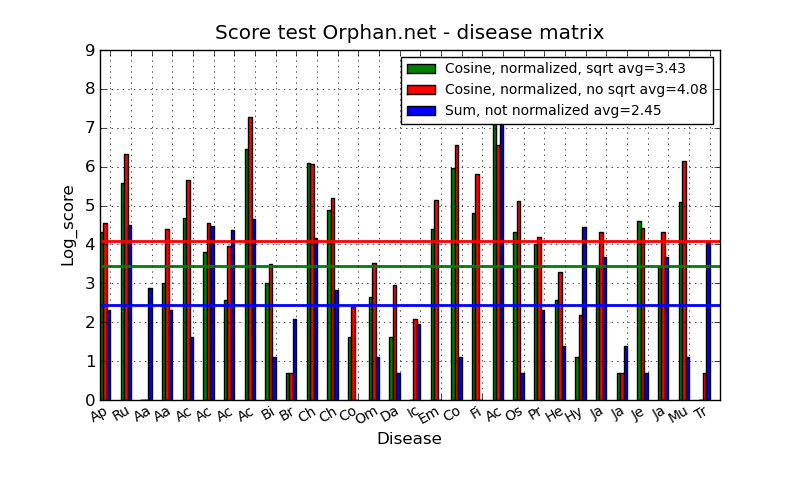
\includegraphics[width=0.9\textwidth]{barcharts/diseaseMatrix_orphan_hist_NOTnorm_3000_s_cos_sqrt_cos_sum_nn.png}
%%         \end{center}
%%         \caption{Test of non-stemmed mean, median and max using normalization and cosine}
%%         \label{Dendro_cat_scratch_disease}
%% \end{figure}


%% \subsection{The reduced semantic space and keyword extraction}
\\
To be written...




\subsection{On overview article noise and concensus normalization\label{Overview}}

Overview articles
Unfortunately there is overview articles that can pollute the search results and if overview articles are found in many of the top scoring diseases, it could present a problem. When we run the concensus method as described in the \ref{CosineScore}, an overview article would potentially get an unfair high score since it gets summed up to 240 times. Though overview articles represents an element of noise, the normalization of the vectors in the vector space model should in theory down weight the highly summed documents. We also tested to the most common overview article (240 occurrences), to see if it could be a problem, using the Orpha.net disease cases among top 3000 (documents). The overview article was present in less than 1 out of 8 searches which is not a significant amount. The disease matrix on the other hand is less prone to the same problem, as it summarizes all information about a disease into one vector. \\

Concensus normalization
During a point in the testing of the term document matrices, we got the idea to try and divide each label with the number of documents it had been summed over. This could in theory normalize the label in the top score of returned results, as labels being over-represented in e.g. the bottom of the top score list would be weighted down. However, as this might be a good theoretical idea, it did not quite amount ot anything useful. The results for running this on the stemmed term document matrix, using the cosine measures, is: \\

Mean: [99, 210, 804, 1216, 507, 667, 167, 309, 502, 50, 330, 695, 424] \\
Median: [1036, 989, 1432, 948, 668, 1301, 1315, 1687, 1429, 1233, 1696, 1494, 1322] \\
Max: [1034, 989, 1447, 1084, 635, 1284, 1293, 1687, 1414, 1233, 1696, 1491, 1321] \\

It does not take a bar chart to see that these values are pretty off the top 20. The idea might be good enough but it would have to be on a different model or data set than the one we use.
